\documentclass[11pt,a4paper]{article}

% ----------------------------------------------------------------------------
% FlowSight — Technical Documentation
% ----------------------------------------------------------------------------

\usepackage[utf8]{inputenc}
\usepackage[T1]{fontenc}
\usepackage[margin=1in]{geometry}
\usepackage{lmodern}
\usepackage{microtype}
\usepackage{graphicx}
\usepackage{xcolor}
\usepackage{enumitem}
\usepackage{booktabs}
\usepackage{longtable}
\usepackage{tikz}
\usetikzlibrary{shapes.geometric, arrows.meta, positioning, fit, backgrounds, calc}
\usepackage{listings}
\usepackage{hyperref}

\definecolor{accent}{HTML}{0F6FAD}
\definecolor{panel}{HTML}{F1F5F9}
\definecolor{codebg}{HTML}{F8FAFC}
\definecolor{kw}{HTML}{0F6FAD}
\definecolor{cmt}{HTML}{64748B}
\definecolor{str}{HTML}{15803D}

\hypersetup{
  colorlinks=true,
  linkcolor=accent,
  urlcolor=accent,
  citecolor=accent
}

\lstset{
  basicstyle=\ttfamily\small,
  backgroundcolor=\color{codebg},
  keywordstyle=\color{kw}\bfseries,
  commentstyle=\color{cmt}\itshape,
  stringstyle=\color{str},
  frame=single,
  rulecolor=\color{panel},
  breaklines=true,
  showstringspaces=false,
  columns=fullflexible,
  numbers=left,
  numberstyle=\tiny\color{cmt},
  xleftmargin=2em,
  framexleftmargin=1.5em
}

\newcommand{\code}[1]{\texttt{\small #1}}

\title{\textbf{FlowSight}\\[2mm]
  \large AI-powered V2X Traffic Intelligence\\[1mm]
  \normalsize Technical Documentation}
\author{Full-Stack Engineering Assessment}
\date{June 2026}

\begin{document}
\maketitle
\tableofcontents
\newpage

% ============================================================================
\section{Objective}
% ============================================================================
FlowSight is a web application that presents traffic data through interactive
charts and an interactive congestion map. It satisfies four functional
requirements --- an interactive \emph{country-wise traffic} chart and an
interactive \emph{vehicle-type distribution} chart on the front end; a REST API
that serves the data; a relational database that stores and allows updates to
the data; and a documented strategy for scaling from 5 to 50 to 500 requests per
second (RPS).

Beyond the brief, FlowSight adds a number of features that make the product feel
like a real operations dashboard: server-side filtering with a date range;
real-time updates over WebSockets; KPI summary cards with a live trend
indicator; an interactive \emph{Greater Vancouver} congestion map with a
time-travel slider, incident impact radii and border-crossing wait times; an
overall traffic-status badge; a top-congested-routes panel; and live
notification toasts. It also ships with containerisation, a CI pipeline, and
unit tests on both ends.

% ============================================================================
\section{Technology Stack}
% ============================================================================
\begin{center}
\begin{tabular}{@{}ll@{}}
\toprule
\textbf{Layer} & \textbf{Technology} \\
\midrule
Front end        & Angular 17 (standalone components), Chart.js 4 \\
Mapping          & Leaflet 1.9 + OpenStreetMap tiles \\
Real-time client & \code{@microsoft/signalr} \\
Back end         & .NET 8 ASP.NET Core Web API \\
Data access      & Entity Framework Core 8 (Npgsql provider) \\
Real-time server & ASP.NET Core SignalR \\
Database         & PostgreSQL 16 \\
Containerisation & Docker, Docker Compose \\
CI/CD            & GitHub Actions \\
Testing          & xUnit (back end), Jasmine + Karma (front end) \\
\bottomrule
\end{tabular}
\end{center}

\noindent The stack was chosen to match the requested .NET + Angular pairing
while staying close to the assessment's preferences (a relational database;
a well-supported framework). PostgreSQL is paired with EF Core via the mature
Npgsql provider, giving migrations, LINQ-to-SQL translation, and strong typing.

% ============================================================================
\section{System Architecture}
% ============================================================================
The system follows a conventional three-tier design with an additional
real-time channel running alongside the request/response path.

\begin{center}
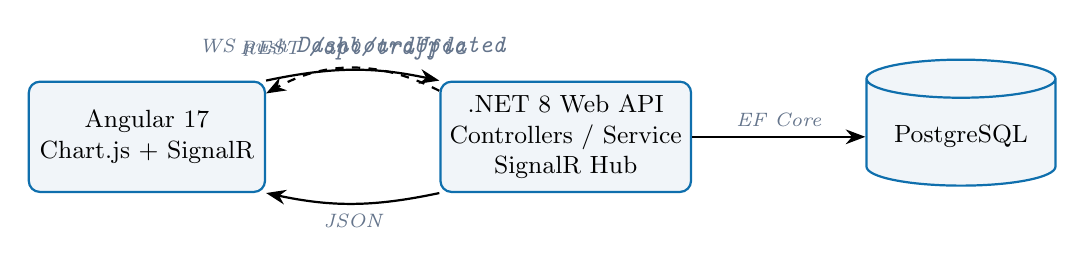
\begin{tikzpicture}[
  node distance=14mm and 22mm,
  box/.style={draw=accent, thick, rounded corners, fill=panel,
              minimum width=30mm, minimum height=14mm, align=center, font=\small},
  db/.style={draw=accent, thick, cylinder, shape border rotate=90,
             aspect=0.25, fill=panel, minimum width=24mm, minimum height=16mm,
             align=center, font=\small},
  arr/.style={-{Stealth[length=2.5mm]}, thick},
  lbl/.style={font=\scriptsize\itshape, color=cmt}
]
  \node[box] (fe) {Angular 17\\Chart.js + SignalR};
  \node[box, right=of fe] (api) {.NET 8 Web API\\Controllers / Service\\SignalR Hub};
  \node[db, right=of api] (db) {PostgreSQL};

  \draw[arr] (fe.north east) to[bend left=12]
        node[lbl, above]{REST \code{/api/traffic}} (api.north west);
  \draw[arr] (api.south west) to[bend left=12]
        node[lbl, below]{JSON} (fe.south east);
  \draw[arr, dashed] (api.160) to[bend right=28]
        node[lbl, above]{WS push \code{DashboardUpdated}} (fe.20);

  \draw[arr] (api.east) -- node[lbl, above]{EF Core} (db.west);
\end{tikzpicture}
\end{center}

\subsection{Request flow}
\begin{enumerate}[noitemsep]
  \item On load, the Angular app calls \code{GET /api/traffic/filters} to
        populate the country and vehicle-type dropdowns, and
        \code{GET /api/traffic} for the initial chart data.
  \item The controller delegates to \code{TrafficService}, which builds two
        aggregate queries (grouped sums) and returns a compact payload.
  \item All grouping and filtering is executed in SQL by PostgreSQL, so the
        response carries only the aggregated points the charts need.
\end{enumerate}

\subsection{Real-time flow}
\begin{enumerate}[noitemsep]
  \item The browser opens a SignalR connection to \code{/hubs/traffic}.
  \item When a new record is posted to \code{POST /api/traffic}, the service
        persists it, recomputes the dashboard, and the controller broadcasts it
        to all clients via \code{IHubContext}.
  \item Each client receives the \code{DashboardUpdated} event and re-renders
        both charts without a page reload.
\end{enumerate}

% ============================================================================
\section{Data Model}
% ============================================================================
The domain splits into two areas. The \textbf{analytics} area has two reference
tables (\code{Countries}, \code{VehicleTypes}) and one fact table
(\code{TrafficRecords}) that drive the dashboard charts. The \textbf{live-map}
area adds four tables --- \code{RoadSegments}, \code{CongestionReadings},
\code{Incidents} and \code{BorderWaits} --- that drive the Greater Vancouver map.

\begin{center}
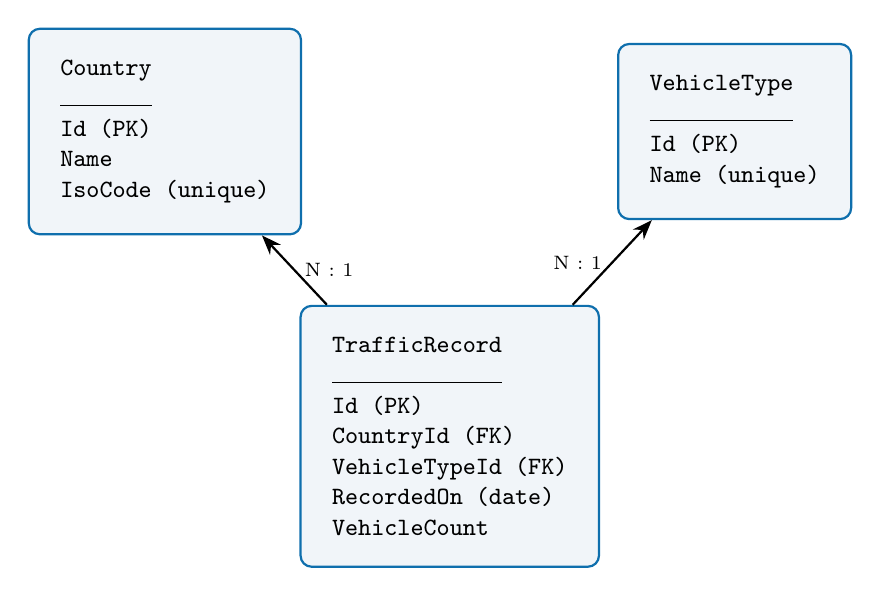
\begin{tikzpicture}[
  ent/.style={draw=accent, thick, rounded corners, fill=panel, align=left,
              font=\small\ttfamily, inner sep=4mm},
  rel/.style={-{Stealth[length=2.5mm]}, thick}
]
  \node[ent] (c) {\textbf{Country}\\\hrulefill\\Id (PK)\\Name\\IsoCode (unique)};
  \node[ent, right=40mm of c] (v) {\textbf{VehicleType}\\\hrulefill\\Id (PK)\\Name (unique)};
  \node[ent, below=22mm of $(c)!0.5!(v)$] (t)
        {\textbf{TrafficRecord}\\\hrulefill\\Id (PK)\\CountryId (FK)\\VehicleTypeId (FK)\\RecordedOn (date)\\VehicleCount};

  \draw[rel] (t) -- node[font=\scriptsize, right]{N : 1} (c);
  \draw[rel] (t) -- node[font=\scriptsize, left]{N : 1} (v);
\end{tikzpicture}
\end{center}

\subsection{Tables}
\begin{longtable}{@{}lll@{}}
\toprule
\textbf{Column} & \textbf{Type} & \textbf{Notes} \\
\midrule
\endhead
\multicolumn{3}{@{}l}{\textbf{Countries}}\\
Id      & integer (identity) & primary key \\
Name    & varchar(100)       & required \\
IsoCode & varchar(3)         & unique, e.g. \code{ARE} \\
\midrule
\multicolumn{3}{@{}l}{\textbf{VehicleTypes}}\\
Id   & integer (identity) & primary key \\
Name & varchar(50)        & unique, e.g. \code{Car} \\
\midrule
\multicolumn{3}{@{}l}{\textbf{TrafficRecords}}\\
Id            & integer (identity) & primary key \\
CountryId     & integer (FK)       & cascade delete \\
VehicleTypeId & integer (FK)       & cascade delete \\
RecordedOn    & date               & observation date \\
VehicleCount  & integer            & aggregated count \\
\midrule
\multicolumn{3}{@{}l}{\textbf{RoadSegments}}\\
Id        & integer (identity) & primary key \\
Name      & varchar(120)       & corridor name \\
PathJson  & text               & JSON \code{[lat,lng]} polyline \\
Capacity  & integer            & reference throughput (veh/hr) \\
\midrule
\multicolumn{3}{@{}l}{\textbf{CongestionReadings}}\\
Id            & integer (identity) & primary key \\
RoadSegmentId & integer (FK)       & cascade delete \\
HourBucket    & integer            & 6, 12, 18 or 22 \\
Volume        & integer            & observed vehicles/hr \\
\midrule
\multicolumn{3}{@{}l}{\textbf{Incidents}}\\
Id           & integer (identity) & primary key \\
Title, Description & varchar       & incident detail \\
Lat, Lng     & double precision   & location \\
RadiusMeters & integer            & impact radius \\
Severity     & varchar(20)        & Low / Medium / High \\
HourBucket   & integer            & active hour \\
\midrule
\multicolumn{3}{@{}l}{\textbf{BorderWaits}}\\
Id          & integer (identity) & primary key \\
Name        & varchar(80)        & crossing name \\
Lat, Lng    & double precision   & location \\
HourBucket  & integer            & 6, 12, 18 or 22 \\
WaitMinutes & integer            & southbound wait \\
\bottomrule
\end{longtable}

\subsection{Indexes}
A composite index on \code{(CountryId, VehicleTypeId, RecordedOn)} and a
single-column index on \code{RecordedOn} support the filtered aggregation and
date-range queries. The map tables are indexed on
\code{(RoadSegmentId, HourBucket)} and on \code{HourBucket} so a single-hour
lookup is cheap. Unique indexes on \code{IsoCode} and \code{VehicleType.Name}
guarantee reference-data integrity.

\subsection{Seed data}
The seeder is idempotent: it inserts each reference row only if it is missing and
backfills traffic records for any country that has none, so an already-seeded
database picks up new entries (such as Canada) on the next run without a reset.
All values are generated deterministically (no randomness), so every environment
produces identical charts and maps.

\begin{lstlisting}[language=,caption={Seeded data}]
Countries     : Canada, United States, United Arab Emirates,
                Germany, India, Japan, United Kingdom
VehicleTypes  : Car, Truck, Bus, Motorcycle, Bicycle
Snapshot dates: 2026-06-01, 2026-06-05, 2026-06-09
Map (Greater Vancouver):
  8 road segments x 4 hour buckets of congestion readings,
  3 incidents, 2 border crossings (Peace Arch, Aldergrove).
\end{lstlisting}

% ============================================================================
\section{Backend API}
% ============================================================================
\subsection{Endpoints}
\begin{longtable}{@{}llp{72mm}@{}}
\toprule
\textbf{Method} & \textbf{Route} & \textbf{Purpose} \\
\midrule
\endhead
GET  & \code{/api/traffic}         & Aggregated dashboard data. Optional query
       parameters: \code{countryId}, \code{vehicleTypeId}, \code{from},
       \code{to}. \\
GET  & \code{/api/traffic/filters} & Lists countries and vehicle types for the
       filter controls. \\
POST & \code{/api/traffic}         & Ingests one traffic record and broadcasts
       the refreshed dashboard. \\
GET  & \code{/api/map}             & Live-map data for an hour bucket
       (\code{?hour=6|12|18|22}): road segments with congestion level and
       estimated delay, incidents, and border-crossing waits. \\
WS   & \code{/hubs/traffic}        & SignalR hub; emits \code{DashboardUpdated}. \\
\bottomrule
\end{longtable}

\subsection{Response shape}
\begin{lstlisting}[language=,caption={\code{GET /api/traffic} response}]
{
  "countryTraffic":      [ { "label": "United States", "value": 5120 }, ... ],
  "vehicleDistribution": [ { "label": "Car", "value": 9800 }, ... ],
  "totalVehicles": 24310,
  "trendPercent": 3.2,      // change vs the previous snapshot date
  "hasTrend": true
}
\end{lstlisting}

\begin{lstlisting}[language=,caption={\code{GET /api/map?hour=18} response (excerpt)}]
{
  "hour": 18,
  "segments": [ { "name": "Highway 1 - Port Mann Bridge",
                  "path": [[49.21,-122.80], ...],
                  "volume": 6300, "capacity": 6000,
                  "level": "heavy", "delayMinutes": 14 }, ... ],
  "incidents": [ { "title": "Multi-vehicle collision",
                   "lat": 49.22, "lng": -122.79,
                   "radiusMeters": 1200, "severity": "High" } ],
  "borders":   [ { "name": "Peace Arch (Douglas)",
                   "waitMinutes": 50, "level": "heavy" } ]
}
\end{lstlisting}

\subsection{Aggregation logic}
The service applies the optional filters, then groups the fact table twice ---
once by country and once by vehicle type --- summing \code{VehicleCount}. Both
queries run \code{AsNoTracking} for read performance and translate to a single
SQL \code{GROUP BY} each.

\begin{lstlisting}[language=,caption={Core aggregation (C\#, simplified)}]
var countryTraffic = await filtered
    .GroupBy(r => r.Country.Name)
    .Select(g => new ChartPoint(g.Key, g.Sum(r => (long)r.VehicleCount)))
    .OrderByDescending(p => p.Value)
    .ToListAsync();
\end{lstlisting}

\subsection{Updating data}
Records are created through \code{POST /api/traffic}. Because the same service
layer is used by both reads and writes, a write is immediately reflected in the
next aggregation and pushed live to every connected client.

% ============================================================================
\section{Frontend}
% ============================================================================
The Angular application is built from standalone components:

\begin{itemize}[noitemsep]
  \item \code{FilterBarComponent} --- country, vehicle and date-range controls
        that emit a filter object on \emph{Apply}.
  \item \code{KpiCardsComponent} --- summary statistic cards (total vehicles with
        a trend arrow, counts, top country, top vehicle).
  \item \code{CountryChartComponent} --- a Chart.js chart with a bar/line toggle.
  \item \code{VehicleChartComponent} --- a Chart.js doughnut chart with
        percentage tooltips.
  \item \code{LiveFeedComponent} --- a connection indicator and a button that
        posts a sample event to demonstrate real-time updates.
  \item \code{LiveConditionsComponent} --- the traffic-status badge and
        top-congested-routes list (driven by \code{/api/map}).
  \item \code{MapDashboardComponent} --- the Leaflet map, time-travel slider and
        incident overlays.
  \item \code{BorderWidgetComponent} --- the border-crossing wait-time card.
  \item \code{AppComponent} --- composes the above behind a Dashboard/Live-Map
        tab switch, owns the current filter and toast notifications, and
        subscribes to both the REST service and the SignalR stream.
\end{itemize}

\noindent Three injectable services isolate I/O: \code{TrafficService} and
\code{MapService} (REST) and \code{RealtimeService} (SignalR). The API base URL
is supplied through an injection token, so it can be swapped per environment
without touching component code. The layout is responsive --- charts and panels
sit side by side on wide screens and stack on narrow ones.

% ============================================================================
\section{Real-Time Updates}
% ============================================================================
SignalR provides a managed abstraction over WebSockets with automatic fallback
and reconnection. The server exposes an empty \code{TrafficHub}; broadcasting is
driven from the controller through \code{IHubContext<TrafficHub>}, which keeps
the hub itself free of business logic.

\begin{lstlisting}[language=,caption={Broadcast on ingest (C\#)}]
var record = await _service.AddRecordAsync(dto, ct);
var dashboard = await _service.GetDashboardAsync(new TrafficQuery(), ct);
await _hub.Clients.All.SendAsync("DashboardUpdated", dashboard, ct);
\end{lstlisting}

\noindent On the client, \code{RealtimeService} exposes the pushes as an RxJS
\code{Observable}, which \code{AppComponent} subscribes to and uses to refresh
the charts.

% ============================================================================
\section{Live Traffic Map}
% ============================================================================
The \emph{Live Map} tab renders an interactive Leaflet map of Greater Vancouver.
It is intentionally a different zoom level from the dashboard: the dashboard is a
country-level overview, while the map is a city-level detail view of one
location, giving an overview-then-drill-down narrative.

\subsection{Congestion colouring}
Each \code{RoadSegment} is drawn as a polyline coloured by its congestion level.
The level is derived server-side from the volume-to-capacity ratio: below 50\,\%
is \emph{low} (green), below 85\,\% is \emph{moderate} (amber), and above that is
\emph{heavy} (red). The API also returns an estimated \code{delayMinutes} per
segment, scaled from the same ratio.

\subsection{Time-travel slider}
A slider steps through four hour buckets (6\,am, 12\,pm, 6\,pm, 10\,pm). Each
change re-fetches \code{/api/map?hour=...} and redraws the overlays, so the user
can watch congestion build through the morning and evening peaks. Seeded volumes
follow a realistic daily curve (rush at 6 and 18, quiet overnight).

\subsection{Incidents and border crossings}
Incidents are drawn as a translucent circle (the impact radius) with a clickable
centre marker. A toggle hides or shows them. The \code{BorderWidgetComponent}
lists southbound wait times for the Peace Arch and Aldergrove crossings, colour
coded by severity, updating with the slider.

% ============================================================================
\section{Dashboard Intelligence}
% ============================================================================
Several touches make the dashboard read like a live operations console; all
figures are computed from real data rather than hard-coded.

\begin{itemize}[noitemsep]
  \item \textbf{KPI trend indicator.} The total-vehicles card shows a green/red
        arrow and percentage. The backend computes this as the change in total
        volume between the two most recent snapshot dates in scope
        (\code{trendPercent}), and omits it when fewer than two dates are
        available.
  \item \textbf{Traffic-status badge.} \code{LiveConditionsComponent} averages
        the current segment load into a four-level status --- Normal (green),
        Moderate (yellow), Busy (orange), Congested (red).
  \item \textbf{Top congested routes.} The same panel ranks road segments and
        border crossings by delay/wait minutes and lists the worst offenders.
  \item \textbf{Live toasts.} When a SignalR update arrives, the client compares
        the new total against the previous one and shows a toast with the real
        delta (e.g.\ ``+287 vehicles detected (+0.6\%)'').
\end{itemize}

% ============================================================================
\section{Scalability: 5 to 50 to 500 RPS}
% ============================================================================
The API is stateless, which is the key property that makes horizontal scaling
possible. The plan below grows the system in three stages.

\subsection{5 RPS --- single instance}
A single API process and a single PostgreSQL instance comfortably serve this
load. The relevant work here is correctness and baseline efficiency: indexed
queries (already in place), EF Core connection pooling, and \code{AsNoTracking}
reads. Vertical headroom is ample.

\subsection{50 RPS --- scale out and cache}
\begin{itemize}[noitemsep]
  \item \textbf{Multiple API replicas} behind a load balancer. Because the API
        holds no per-request state, replicas are interchangeable.
  \item \textbf{Redis response cache} on the aggregation endpoint. Dashboard
        data changes far less often than it is read, so short-lived caching
        (with cache invalidation on ingest) removes most database load.
  \item \textbf{SignalR Redis backplane} so a push from any replica reaches
        clients connected to any other replica.
  \item \textbf{Connection-pool tuning} and PgBouncer in front of PostgreSQL.
\end{itemize}

\subsection{500 RPS --- elastic and distributed}
\begin{itemize}[noitemsep]
  \item \textbf{Auto-scaling} of API pods on Kubernetes (Horizontal Pod
        Autoscaler keyed on CPU/RPS).
  \item \textbf{Read replicas} for PostgreSQL; the read-heavy aggregation
        traffic is routed to replicas while writes go to the primary.
  \item \textbf{Materialized views} (or a pre-aggregated summary table refreshed
        on ingest) so the hottest queries become simple lookups.
  \item \textbf{CDN} for the static Angular bundle, removing front-end delivery
        from the origin entirely.
  \item \textbf{Message queue} (e.g. Kafka/RabbitMQ) in front of ingestion to
        absorb write spikes and decouple producers from the database.
  \item \textbf{Observability} --- metrics, tracing and autoscaling alarms to
        keep the system within its latency budget.
\end{itemize}

\begin{center}
\begin{tabular}{@{}llll@{}}
\toprule
 & \textbf{5 RPS} & \textbf{50 RPS} & \textbf{500 RPS} \\
\midrule
API        & 1 instance     & N replicas + LB      & autoscaled pods \\
Cache      & none           & Redis               & Redis + materialized views \\
Database   & single         & single + PgBouncer  & primary + read replicas \\
Real-time  & in-process     & Redis backplane     & Redis backplane \\
Static     & origin         & origin              & CDN \\
Ingestion  & direct         & direct              & message queue \\
\bottomrule
\end{tabular}
\end{center}

% ============================================================================
\section{Testing}
% ============================================================================
\subsection{Backend (xUnit)}
\code{TrafficServiceTests} uses the EF Core in-memory provider to verify the
aggregation logic in isolation: unfiltered totals, filtering by country,
date-range exclusion, and that a newly added record is counted. Each test runs
against a fresh database instance.

\subsection{Frontend (Jasmine + Karma)}
\code{TrafficService} is tested with \code{HttpTestingController} to confirm the
correct URLs and query parameters are produced. \code{FilterBarComponent} is
tested for its emit-on-apply and reset behaviour.

% ============================================================================
\section{Deployment}
% ============================================================================
\subsection{Docker Compose}
A single \code{docker compose up --build} starts three services: PostgreSQL, the
API (which migrates and seeds on startup), and the Angular app served by nginx.
A health check on the database gates the API start-up so migrations never race
an unready database.

\begin{center}
\begin{tabular}{@{}lll@{}}
\toprule
\textbf{Service} & \textbf{Image / build} & \textbf{Host port} \\
\midrule
db       & \code{postgres:16-alpine}    & 5432 \\
api      & \code{backend/Dockerfile}    & 5000 $\rightarrow$ 8080 \\
frontend & \code{frontend/Dockerfile}   & 8081 $\rightarrow$ 80 \\
\bottomrule
\end{tabular}
\end{center}

\subsection{CI pipeline (GitHub Actions)}
On every push and pull request to \code{main}, two parallel jobs run. The
back-end job restores, builds and runs \code{dotnet test}; the front-end job
installs dependencies, runs the Jasmine suite headless, and produces a
production build. A green pipeline therefore proves both halves compile and pass
their tests.

% ============================================================================
\section{Running the Project}
% ============================================================================
\textbf{With Docker:}
\begin{lstlisting}[language=bash]
docker compose up --build
# Frontend  -> http://localhost:8081
# API/Swagger -> http://localhost:5000/swagger
\end{lstlisting}

\textbf{Locally:}
\begin{lstlisting}[language=bash]
# Backend
cd backend && dotnet run --project FlowSight.Api

# Frontend
cd frontend/flowsight-web && npm install && npm start
\end{lstlisting}

% ============================================================================
\section{Design Decisions and Trade-offs}
% ============================================================================
\begin{itemize}[noitemsep]
  \item \textbf{Aggregate in the database, not the client.} Grouping and summing
        in SQL keeps payloads tiny and pushes work to the layer best suited for
        it.
  \item \textbf{Stateless API.} The single most important decision for
        scalability; it makes every later scaling step (replicas, autoscaling)
        straightforward.
  \item \textbf{Broadcast from the controller, not the hub.} Keeps the hub thin
        and the business logic in one place (the service layer).
  \item \textbf{Injection token for the API URL.} Environment configuration
        without code changes.
  \item \textbf{Minimal, deterministic seed data.} Enough to exercise both
        charts and every filter, reproducible across environments, with no
        bloat.
  \item \textbf{Honest, computed metrics.} Trends, status and delays are derived
        from the data, not invented, so the figures hold up under inspection.
\end{itemize}

\vspace{4mm}
\noindent\rule{\linewidth}{0.4pt}\\[1mm]
\small This document describes the structure and reasoning behind the FlowSight
codebase included in the same repository.

\end{document}
